% Standard template book
\documentclass[11pt, a4paper, oneside]{book}

%%%%%%%%%%%%%%%%%%%%%%%%%%%%%
% Packages
%%%%%%%%%%%%%%%%%%%%%%%%%%%%%

% Better looking urls
\usepackage[hyphens]{url}

% During testing to se all the margins
% \usepackage[showframe]{geometry}
% Package parskip is supposed to fix whitespaces in list
% and other environments when you alter the \parskip setting.
% https://en.wikibooks.org/wiki/LaTeX/Paragraph_Formatting
\usepackage{parskip}

% Remove indentation of first line in each paragraph
\setlength{\parindent}{0cm} % Default is 15pt.

% Add whitespace between paragraphs
\setlength{\parskip}{3mm}
%\setlength{\parskip}{3mm plus4mm minus3mm}

% Alter headers and footers
\usepackage[pagestyles]{titlesec}
\newpagestyle{footerPageNumberMiddle}{\setfoot[\thepage][][]{}{\thepage}{}}

% Adding \figure support
\usepackage{graphicx}

% Source code support
\usepackage{listings}

% Math support
\usepackage{amsmath} % Math
\usepackage{amsthm} % Theorems and proofs

% Theorems details
% http://www.sharelatex.com/learn/Theorems_and_proofs
\theoremstyle{definition}
\newtheorem{defi}{Definition}
\newtheorem{theorem}{Theorem}[section]
\newtheorem{lemma}[theorem]{Lemma}

% Change whitespace above theorems
\makeatletter
\def\thm@space@setup{%
    \thm@preskip=10pt \thm@postskip=0pt
}
\makeatother

% Add support for list of abbreviations
\usepackage{nomencl}
\makenomenclature
\setlength\nomlabelwidth{3cm} % Change this value to align the list of abbrev.

% Caption support in figures
% with sub-figures
\usepackage[hypcap=true]{caption}
\usepackage[hypcap=true,list=true,listformat=simple]{subcaption}

% Add links within the PDF
% All links are turned into booksmarks as well
\usepackage[bookmarks, hidelinks]{hyperref}

% Make sure hyperlinks to figures link to top of image
% and not to the caption.
\usepackage[all]{hypcap}

% Make it possible to add bookmarks without entries in the
% table of content.
\usepackage{bookmark}

% Specifiy table of content settings
\setcounter{tocdepth}{1}

%%%%%%%%%%%%%%%%%%%%%%%%%%%%%
% Document start and frontmatter
%%%%%%%%%%%%%%%%%%%%%%%%%%%%%
\begin{document}
\frontmatter

\cleardoublepage
\pdfbookmark{Front page}{Front page}
% Title
\title{{\large \uppercase{Master Thesis}} \\[0.4cm]
{ \huge \bfseries Model-checked,\\Space Plug-and-Play Architecture Local Subnet
Adaptation, implemented in Ada with Ravenscar restrictions} \\[0.4cm]
}


% Author
\author{\emph{Author} \\
Christoffer Holmstedt\\[1cm]
\begin{tabular}{ p{7cm} r }
\textit{Supervisor} & \textit{Examiner} \\
Adj. Prof. Fredrik Bruhn, PhD & Prof.~Kristina Lundqvist
\end{tabular}\\[4cm]
\uppercase{\textbf{M\"{a}lardalen University}} \\
School of Innovation, Design and Engineering
}

% % Title
% \cleardoublepage
% \pdfbookmark{Front page}{Front page}
% \title{Model-checked, Space plug-and-play Architecture Local Subnet Adaptation,
% implemented in Ada with Ravenscar restrictions}
% 
% % Author
% \author{Christoffer Holmstedt}

\maketitle

%%%%%%%%%%%%%%%%%%%%%%%%%%%%%
% Abstract
%%%%%%%%%%%%%%%%%%%%%%%%%%%%%

\cleardoublepage
\pdfbookmark{Abstract}{Abstract}
\chapter*{Abstract}
\thispagestyle{empty} % No page numbering on this page
Space Plug-and-Play Architecture (SPA) is a set of standards to make it easier
to build small satellites. Focus is put on improving the integration phase and
the time consuming validation and verification process by introducing
plug-and-play functionality. From mission call-up to operational satellite it
should only take six days.

A SPA network consists of several different types of subnets with different
pros and cons. For each processing node there must be one Local Subnet Manager
(SM-L). The SM-L can communicate over different communication protocols
depending on how the respective local subnet is set up, one option is UDP/IP.

In this thesis Ada Protected Objects is presented as a viable option for
inter-process communication instead of UDP/IP in a SPA network. This thesis
present the initial work towards a SPA Local Subnet Adaptation that builds on
language constructs in Ada such as Ada Tasks and Protected Objects.  The system
design and implementation is verified deadlock free with UPPAAL but shows
indications of livelock possibilities. The severity of these livelock
situations is discussed in the conclusion.

% Keywords
\textbf{Keywords:} Space plug-and-play Architecture, SPA, UPPAAL, Timed
automata, Ada, Ravenscar, Unified Common Architecture, UNICA, Virtual Network
Protocol, VNP


%%%%%%%%%%%%%%%%%%%%%%%%%%%%%
% Acknowledgement
%%%%%%%%%%%%%%%%%%%%%%%%%%%%%

% \cleardoublepage
% \pdfbookmark{Acknowledgement}{Acknowledgement}
% \chapter*{Acknowledgement}
\thispagestyle{empty} % No page numbering on this page
TODO


%%%%%%%%%%%%%%%%%%%%%%%%%%%%%
% Table of Content, List of Figures/Tables
%%%%%%%%%%%%%%%%%%%%%%%%%%%%%

\cleardoublepage
\pdfbookmark{\contentsname}{Contents}
\tableofcontents

% \listoffigures
% \addcontentsline{toc}{chapter}{\listfigurename}
% \listoftables
% \addcontentsline{toc}{chapter}{\listtablename}

% List of Abbrevations
% To align the columns change the value further up in this file next
% to loading the nomencl package.
\renewcommand{\nomname}{List of Abbreviations}
\cleardoublepage
\printnomenclature
\addcontentsline{toc}{chapter}{\nomname}

%%%%%%%%%%%%%%%%%%%%%%%%%%%%%
% Mainmatter - The Report
%%%%%%%%%%%%%%%%%%%%%%%%%%%%%

\mainmatter
\pagestyle{footerPageNumberMiddle}
\chapter{Introduction}

\section{Background}
TODO: Summary of the State of the Art.

\section{Problem Statement}
TODO: Definition of the problem statement(s).

TODO: Define the different properties/attributes to be measured when comparing
event-triggered and time-triggered systems.

TODO: Define what is in scope and what is out of scope.

\section{Structure of this report}
TODO: Add one paragraph with information on how the following chapters and
sections are structured. This section title might not be needed for this
paragraph.

\chapter{State of the Art} \label{ch:state_of_the_art}

\section{Space plug-and-play Architecture}
The Air Force Resarch Laboratory (AFRL) Space Vehicle Directorate started a
project referred to as "Space plug-and-play Avionics" in 2004 with the intent
to understand why space systems used in various mission became so complex and
how they can be made easier to assembly \cite{fronterhouse2007, martin2012}.
The solution was to look at plug-and-play systems already available on ground.
An example to this is how USB devices work with laptop and desktop computers in
everyday life. It doesn't matter which keyboard you buy the basic functionality
will work in any computer you plug it into, no matter if it runs Windows, OS X
or a Linux distribution.

"Space plug-and-play Avionics" was released during the 2000-decade as a set of
standards and in an updated version in 2011 renamed to "Space plug-and-play
Architecture" \cite{martin2012}, all standards are available from AIAA
\cite{spa:all}.

\nomenclature{\textbf{AFRL}}{\textbf{Air Force Resarch Laboratory}}

Development and testing of implementations conforming to the standards have
been ongoing since the launch of the program. One project that has been
presented is the PnPSat by Fronterhouse et. al. \cite{fronterhouse2007} and
Martin et. al. \cite{martin2008}. They have demonstrated the first created
plug-and-play satellite and given their view on the problems encountered during
development of both hardware and software. The first plug-and-play satellite
flown on orbit is presented by Martin et. al. \cite{martin2012} where most
parts of the plug-and-play experiement passed all tests one year after launch.

As a critical part of plug-and-play satellite research and development is the
"System Data Model" (SDM) middleware software presented by Sundberg et. al.
\cite{sundberg2006}, previously under the name "Satellite Data Model"
\cite{spa:sdm-source}. The SDM can be viewed in two different ways, as a
middleware or as a "sideware" \cite{fronterhouse2007}, depending on how you
view it. The SDM is one implementation of the SPA standards that manage the
parts of handing out logical addresses to all SPA components, doing network and
data capabilities discovery. The SDM source code has been released under public
domain license \cite{spa:sdm-source}.

\nomenclature{\textbf{SDM}}{\textbf{System Data Model}}

To enable components to be self-describing all SPA components must have a xTEDS
file stored within the component. The xTEDS file include all the information
other components need to understand its capabilities e.g. which interfaces the
component have. The problem at this point arise that multiple vendors start to
create their own interface definitions and all benefits with self-describing
components are lost. This is where the "Common Data Dictionary" (CDD) comes
into play.

\nomenclature{\textbf{CDD}}{\textbf{Common Data Dictionary}}

The first work to create the CDD is described as an informal approach by Pasko
\cite{pasko2011}, instead a more formal approach using RDF is suggested. Pasko
suggests that RDF and RDF Schemas can be used to not only desribe the CDD
formally but also be used to visually represent the CDD with suitable software.

Hansen et. al.  \cite{hansen2012} describes the dictionary as an ontology which
consists of several taxonomies in a hierarchial structure. This means that if
different vendors respectively create a SPA component with a temperature sensor
and a pressure sensor interface the vendors use the CDD to describe the
interfaces with the correct vocabulary. To manage the risk of adding too
many terms in the CDD Lanza et. al. \cite{lanza2010} suggests the forming of a
CDD panel to "[...] serve as a regulatory structure for the CDD". To make it
easier for developers to write xTEDS files with the correct vocabulary and
improve the CDD, Lanza et. al.  \cite{lanza2010} have created a web based tool
to manage the CDD.

One benefit of using XML file structure for the xTEDS is that a XML schema
definition (XSD) can be created and with the help of a XML validating parser
xTEDS can be verified automatically to conform to the xTEDS file format and the
CDD \cite{lanza2010}.

\nomenclature{\textbf{XSD}}{\textbf{XML Schema Definition}}

\section{Model Checking and UPPAAL}
TODO: Start with model checking in general, introduce the concept of timed
finite automata and give examples on how it has been used by others.

TODO: Some notes about UPPAAL and the different forks available.

\section{Internet of Things}
TODO: Do a broad overview of the concept of Internet of Things and the
different standards that are available.

\chapter{Method}\label{ch:method}
\section{Literature study}
The literature study was conducted by selecting different key terms related to
the topics and searching for them in two different search engines. The first
one was Google scholar and the second one was the "Discovery" search engine
available for Mälardalen University's students and employees. The Discovery
search engine search through multiple databases such as IEEE Xplore,
ACM Digital Library and SpringerLink. For searches in the Discovery search
engine only articles with full text available was requested.

In Google scholar the first 20 results were looked into and the first 40
results given by Discovery search engine was looked into. Only results with
full text PDFs were selected from Google Scholar.

A first read through of abstracts was conducted to filter out unrelated
papers and then followed by a read through of introductions and conclusions for
another filtering round. The key terms selected are shown below under
respective topic's section.

\subsection{Space plug-and-play Architecture}
The key terms chosen was "Space plug-and-play Avionics", "Space
plug-and-play Architecture" and "why Space plug-and-play Avionics".

All references from two relatively new reports were looked into as well.

% space plug-and-pay avionics
%AFRL plug and play spacecraft avionics.
%developing an ontology.

\subsection{Dependability and Ada}
\subsection{Model Checking and UPPAAL}
\subsection{Internet of Things}

\section{An Agile Unified Process}
\subsection{Requirements Analysis}
TODO: Write down how I did the requirements analysis and which references I
used for guidance.

\subsection{Design with UML}
TODO: Write down how I did the design and which references I used for guidance.

\subsection{Modeling, validation and verification with UPPAAL}
TODO: Write down how I did the modeling, validation and verification and which
references I used for guidance.

\subsection{Development in Ada}
TODO: Write about the development in Ada and how regression testing was done.
Test-Driven Development was used and so on.

\subsection{An iterative process}
TODO: Mention that the requirements analysis to development in Ada (sections
above) was iterated twice to improve the end result.

\chapter{Space Plug-and-Play Architecture}\label{ch:spa}
Space plug-and-play Architecture (SPA) is a set of standards that define how
different players can create plug-and-play components that can easily be
assembled to form a complete satellite for a specific mission. The standards
are published by American Institute of Aeronatuics and Astronautics (AIAA). The
standards range from how power supply should be handled to how components
communicate in the application layer, focus in this report is put on the
software parts.

To describe how a SPA network works some terminology needs to be defined. All
nodes in a SPA network are called "components", there is no differentiation
between software and hardware components. Each component has a "Component
Universally Unique Identifier" (CUUID) which is 128 bit long. Each component
also has an "Extensible Transducer Electronic Data Sheet" (xTEDS) file that
describes respective components capabilities. To be able to support different
underlying link layer technologies such as Ethernet, Spacewire and one-wire
(I2C), most functionality has been put in the application layer. This means
that a SPA network can be built with any combination of link layer "subnets",
for example a SPA network can consist of two Spacewire subnets and one Ethernet
subnet.

\nomenclature{\textbf{CUUID}}{\textbf{Component Universally Unique Identifier}}

The important concepts to remember is that each SPA component is
connected to one or more SPA subnets, on each SPA subnet there is a subnet
manager (SM-x) that acts as a gateway to other SPA subnets and when SPA subnets
are linked together they form a SPA network. To make things clear, a single SPA
subnet with a CAS, LS and SM-x is also a SPA network.

Another SPA subnet is the SPA Local Subnet. Each processing node that can
have multiple SPA components running on it has a "SPA Local Subnet Manager"
(SM-L).  Components within a processing node should do inter-process
communication over UDP/IP \cite{spa:local-subnet}.

Components communicate with each other with the help of "logical addresses"
that each component recieves during boot up. It is the responsiblity of the
"Central Addressing Service" (CAS) to hand out logical addresses to all
components in the SPA network through the connected Subnet Managers. After a
component receives its logical address it can share its xTEDS file with other
components. It is the responsibility of the "Lookup Service" to keep track of
the capabilities of each component in the SPA network.

To describe what a SPA network can look like figure
\ref{fig:minimal_spa_network} shows a minimal SPA network which consists of a
CAS, LS, a sensor and a monitor application, all running on the same processing
node and in the same local subnet managed by the SM-L.

\begin{figure}[h]
    \centering
    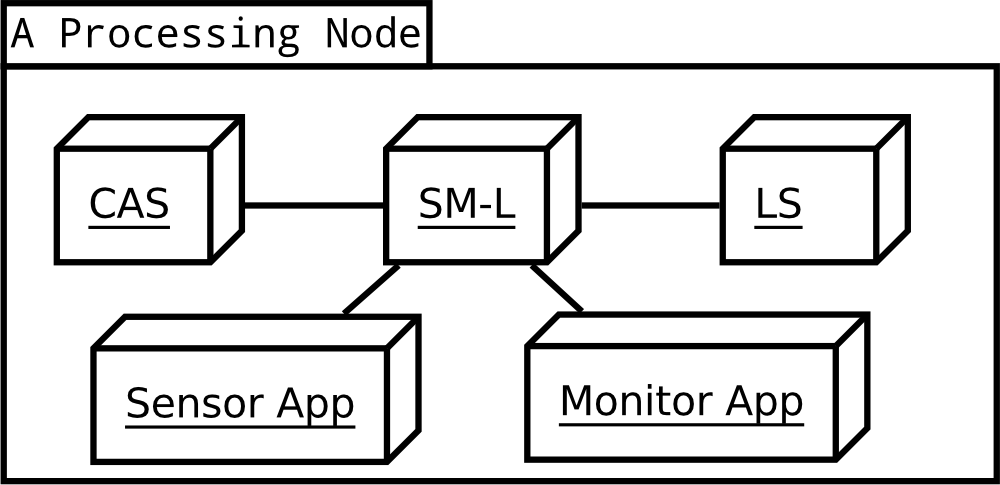
\includegraphics[width=\textwidth]{figures/minimal_spa_network}
    \caption{A processing node running a minimal SPA network.}
    \label{fig:minimal_spa_network}
\end{figure}

A more complex SPA network is shown in figure \ref{fig:complex_spa_network}.
Three different processing nodes are connceted to each other over a
SPA-Ethernet subnet. The CAS, LS and Monitor Application are now running on
different nodes and the sensor application is located on its own embedded
device.

\begin{figure}[h]
    \centering
    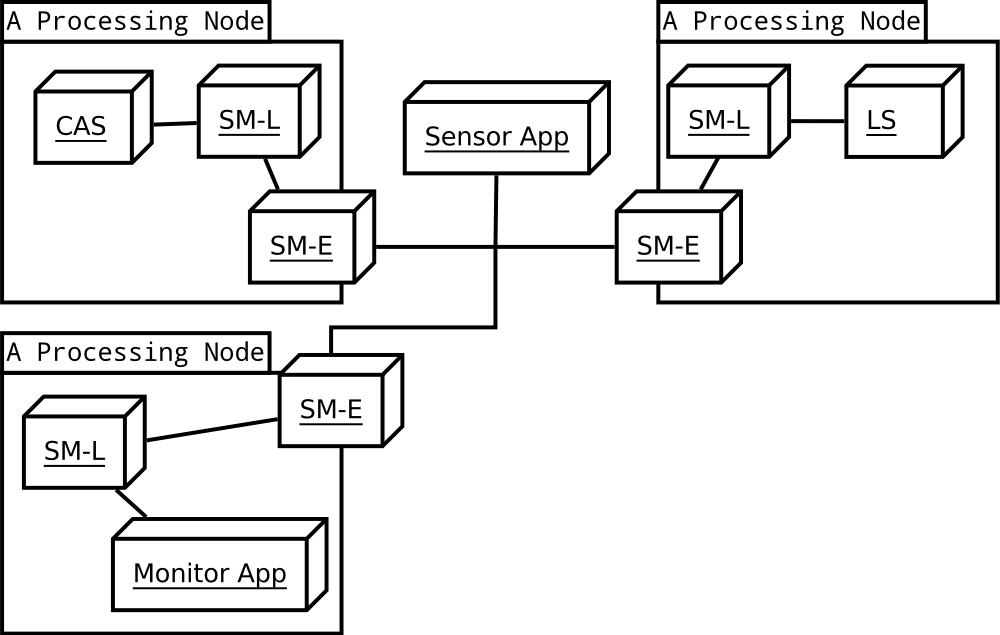
\includegraphics[width=\textwidth]{figures/complex_spa_network}
    \caption{A SPA network with multiple subnets.}
    \label{fig:complex_spa_network}
\end{figure}

For a detailed view on how SPA works the SPA standards is the best source for
information. The SPA standards and drafts that specify software requirements
are the Logical Interface standard \cite{spa:logical-interface}, Networking
standard \cite{spa:networking}, Local Subnet Draft \cite{spa:local-subnet},
Ontology Standard \cite{spa:ontology} and System Capabilities Standard
\cite{spa:system-capabilities}.


% \section{Virtual Network and the Virtual Network Protocol}
% TODO: Finish of with the definition of Virtual Network, Virtual Network
% Protocol and how it relates to SPA.
%
% TODO: Is this needed or should VNP perhaps only be mentioned in context with
% development efforts and code? This would mean that all comments about VN/VNP is
% pushed to the results and conclusion parts...perhaps some in the method.

\chapter{Designing and modeling the system}\label{ch:uppaal_models}
This chapter includes the UPPAAL models in conjunction with corresponding UML
diagrams describing the implementation done in Ada. The UPPAAL models are used
for the validation and verification of the system that it meets the real-time
requirements set on the system. The connection from the UPPAAL models to the
UML diagrams presented here are to show that the implementation corresponds as
close as possible to the models verified.

For presentation purposes only the messages concerning basic functionality
during component and service discovery is presented in this chapter. After the
initial discovery and configuration process have been done the system continue
in normal operation mode with an extra set of SPA message types. Detailed
sequence diagrams over the component and service discovery process is shown in
section \ref{sec:discovery_process}.

\section{First iteration}
The first UPPAAL models were created after designing the basic structure of the
system. Each application will do the same thing which is receive, handle
and send messages. The difference between the applications is which
messages each application understands and which messages the application will
ignore. A processing node will at most have one CAS, one SM-L and one LS
but can have any number of applications running next to them. This inspired the
first iteration of UPPAAL models that the application automaton should be
possible to instantiate multiple times in UPPAAL but the other more specific
models can be used only ones. The basic component overview is shown in figure
\ref{fig:processing_node_overview} which is what the UPPAAL model is to
resemble as close as possible.

\begin{figure}[h]
    \centering
    
\includegraphics[width=\textwidth]{figures/processing_node_overview}
    \caption{A Processing Node overview with core SPA parts.}
    \label{fig:processing_node_overview}
\end{figure}

\subsubsection{A basic application}
The basic functionality of an application is that it should be able to identify
itself on the network, share its capabilities and request information from
other applications. An application is only connected to one subnet at a time.
The limitied functionality of an application makes for a basic two-layered
design where the upper-layer alter its behaviour depending on incoming
message types and the lower layer is only responsible for sending and receiving
messages on its subnet. The application sends out Local\_Hello message during
boot-up and receives a Local\_Ack response, all messages are modeled as
transition between different states. It then receives a logical address with
the Assign\_Address message. As final step it receives a Probe\_Request from
the Lookup Service to share its capabilities. Figure
\ref{fig:iteration1_application} shows the UPPAAL model.

\begin{figure}[h]
    \centering
    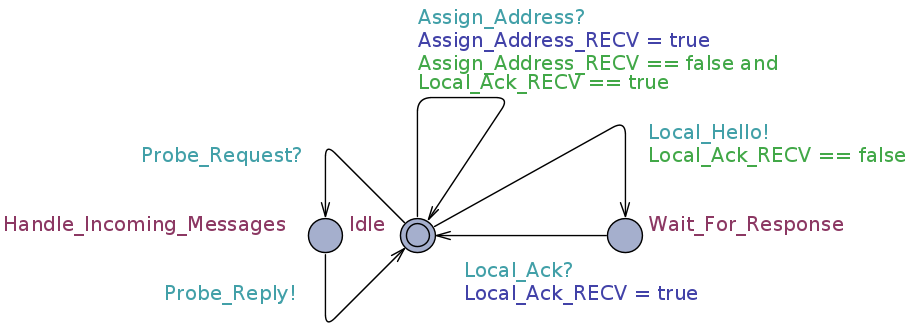
\includegraphics[width=\textwidth]{figures/iteration1_application}
    \caption{UPPAAL model of a first iteration application.}
    \label{fig:iteration1_application}
\end{figure}

\subsubsection{Central Addressing Service (CAS)}
Specifics for the CAS is that it assigns an address to itself so no need for
processing of Assign\_Address messages. As addition to basic application
functionality the CAS sends out address block to the requesting subnet
managers. Figure \ref{fig:iteration1_cas} shows the UPPAAL model.

\begin{figure}[h]
    \centering
    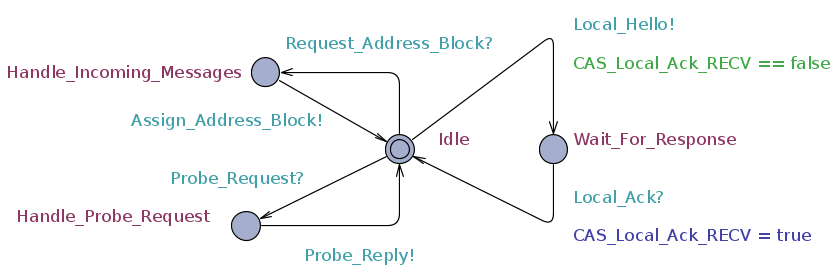
\includegraphics[width=\textwidth]{figures/iteration1_cas}
    \caption{UPPAAL model of a first iteration CAS.}
    \label{fig:iteration1_cas}
\end{figure}

\subsubsection{Lookup Service (LS)}
The additions the LS brings in is the processing of Request\_LS\_Probe,
Probe\_Reply and Probe\_Request messages, for service discovery purposes.
Figure \ref{fig:iteration1_ls} shows the UPPAAL model.

\begin{figure}[h]
    \centering
    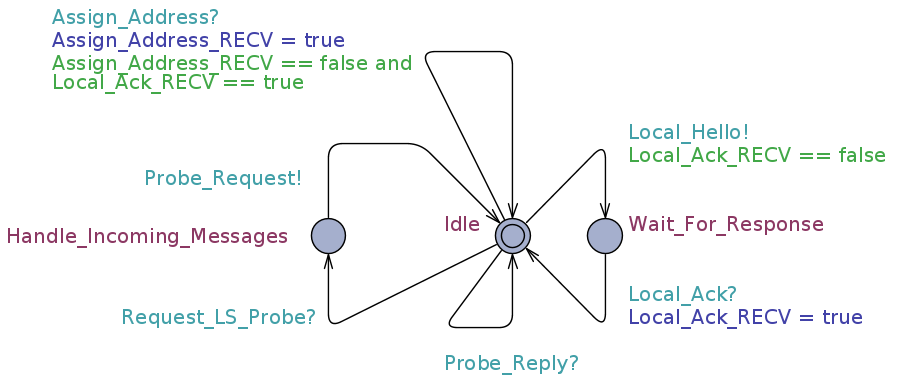
\includegraphics[width=\textwidth]{figures/iteration1_ls}
    \caption{UPPAAL model of a first iteration LS.}
    \label{fig:iteration1_ls}
\end{figure}

\subsubsection{Local Subnet Manager (SM-L)}
In contrast to the other components the Subnet Manager manages most of the
interaction done in the subnet. It's responsible for answering all Local\_Hello
messages during component discovery and replying with an acknowledgement as
well as with an logical address assignment. As a last step it tells the LS to
send out Probe\_Requests to all active components on the subnet.Figure
\ref{fig:iteration1_sm_l} shows the UPPAAL model.

\begin{figure}[h]
    \centering
    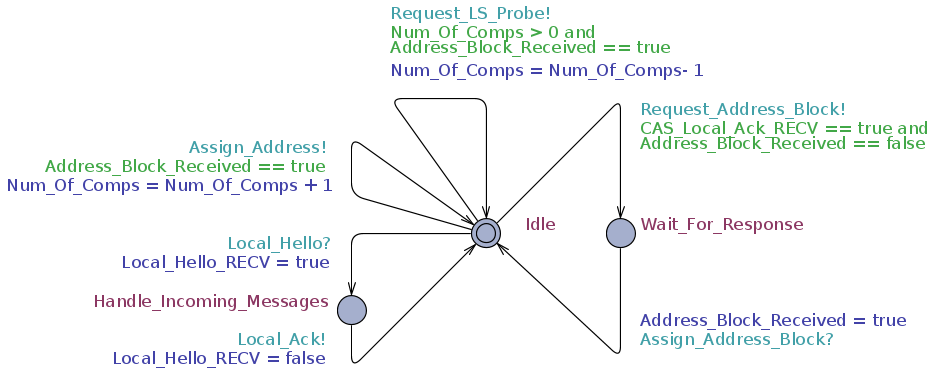
\includegraphics[width=\textwidth]{figures/iteration1_sm_l}
    \caption{UPPAAL model of a first iteration SM-L.}
    \label{fig:iteration1_sm_l}
\end{figure}


\subsubsection{First iteration conclusions}
The CAS, LS and SM-L have specific functionality so they can only be used ones
when setting up a complete network of automata. The application model can be
instantiated multiple times as was the goal. At this level of abstraction
everything looks fine though the main goal with the UPPAAL model is to be able
to verify that the system behaves as aspected and can't reach unknown states or
deadlock. As the first iteration of models only shows the boot-up process it
will eventually reach deadlock when everything is set up. This is a drawback
as it doesn't relate very well with the actual design of the system, that can
have different applications come online and go offline at any time, not just
during initial boot-up. This calls for another iteration and improvement of the
different UPPAAL automata.

Before heading to the second iteration it's time to take a closer look at the
UPPAAL automata and see what other parts need improvements, as it should
resemble the actual system as much as possible.

First of is that the current automatons use transitions to model sent and
received messages. When a transition is taken to send a message the different
automata takes the transition to responed immediatly afterwards. This is more
or less an event-based system which is not how the system should behave.
Instead the second iteration of UPPAAL models should be modeled as a
time-triggered system so responses can be sent later on.

The models only works with a set of eight different message types and in the
current design of the UPPAAL models it's hard to add another type of message.
If possible the second iteration should make it possible to add and remove
specific message types with ease.

As a third improvement time invariants should be added to the different
automata so verification of real-time requirements can be done.

\section{Second iteration}
To improve the UPPAAL models a more detailed design is required of the system.
From the first iteration it's clear that the basic application can be designed
in a generic fashion. The CAS and LS is more specific instantiations of the
basic application and the SM-L has substantial differences. For easier
maintanence of the models during the second iteration it would be valuable if
the UPPAAL models could created in a modular way. Two main models would be the
"basic application" and the "SM-L".

\subsubsection{A basic application}
TODO
\subsubsection{Central Addressing Service (CAS)}
TODO
\subsubsection{Lookup Service (LS)}
TODO
\subsubsection{Local Subnet Manager (SM-L)}
TODO
\subsubsection{Second iteration conclusions}
TODO

\section{Validation and Verification}
TODO: Add comments about time verification and correctness. What are the
verification lines used in UPPAAL to verify the system?

% \section{An event-triggered alternative}
% TODO: All models and comments about an event-triggered alternative.

\chapter{Result}\label{ch:result}
\section{Model verification}
The model presented in chapter \ref{ch:designing_and_modeling} was verified
with the verification queries presented in the same chapter.

\begin{itemize}
    \item For deadlock verification the property was satisfied.
    \item For livelock verification the property was not satisfied.
\end{itemize}

% \section{Time-triggred and event-triggered systems}
% TODO: Write down the different results I found (the properties/attributes to be
% measured must be defined in the problem statement).

\section{Implementation}
The implemented SPA framework code called "Virtual Network Library" is
available on Github at \url{https://github.com/virtualnetwork/vn-lib}. The
modular design is shown in figure \ref{fig:appendix_component_overview} and the
source code compiles with the Ravenscar restrictions. Efforts has also been
made to limit the amount of dynamic memory usage.

Example implementation is available in the "examples" directory in the git
repository.

\chapter{Conclusion}\label{ch:conclusion}
Presented in this thesis report is a model-checked implementation of a new
subnet local adaptation for the Space plug-and-play Architecture, implemented
as the Virtual Network Library \cite{web:github-vn-lib} for the fork of SPA
called "Virtual Network Protocol". Instead of UDP/IP for IPC, Ada Protected
Objects are used to share data between different Ada tasks.

When model-checking a system to verify that it behaves as expected it's
important to get the model to resemble the implementation as close as possible
and the implementation to resemble the model as close possible. It's a network
of two development artifacts that prove that the system behaves according to
specifications. In this thesis the specifications are the SPA standards
and our implementation is the "Virtual Network Library" implementation with
example applications that is verified.

In chapter \ref{ch:designing_and_modeling} the process that took place to reach
the end result when it comes to UPPAAL models and implementation is shown.
Going further with an even more detailed model would go into unnecessary detail
such as how the routing tables were implemented or how the CAS table was
implemented. As the different tables are not going to hold any substancial
amount of data the time to do a lookup in the different tables are
neglectable. This leads to the conclusion that the model's level of abstraction
is about right for the goal with this thesis.

...

TODO: Is both the event- and time-triggered systems verified correcly with the
models and are the models good abstractions from the real-world implementation?
Is event- or time-triggered systems best in this field?

\section{Future research and development}
The major consequence of moving away from UDP/IP as IPC is that the
applications running on the different processing node no longer are modular in
the sense that it's easy to add and remove applications on a processing node in
a running system. When using Ada Protected Objects all applications must be
compiled together into one binary and started at the same time. This leads to
future updates must replace the entire binary and reboot the system. The
trade-off between Ada Protected Objects and a run-time modularity is something
that need to be prioritzed per project basis. For robots or satelites that are
not connected to internet the increased reliability of protected objects may be
a good trade-off. On the other side devices connected to internet that always
must be up to date security wise to protect against intrusions, the modularity
may be prioritized.  An example to this could be a refridgerator that is
connected to internet and a vulnerability is found in it's transport layer
security code. Instead of updating the entire running binary it would be enough
just to update the specific module that expose the vulnerability. Future work
should look into the possibility of keeping some run-time modularity and
introducing Ada Protected Objects.

For closed-circuit networks like remote operated vehicles and some robots,
security may not be that important but for the vast majority of devices
security need to be introduced. As soon as a device is connected to internet
and start to communicate with others it will need some kind of authentication
mechanism to allow access to its own data, it will need authorization mechanism
to be able to differentiate between different other devices regarding which
device should get access to what data. Added to this is transport encryption
(confidentiality) to prevent pervasive monitoring and the possiblitiy of
disclosing private information to active listeners (man-in-the-middle attacks).
How to add security to a SPA network with open access to internet is an
important step forward to make SPA a viable option in the world of Internet of
Things.

When starting this thesis Ada was chosen as programming language because of its
track record with software that must be dependable to high-levels. Different
ISO standards and white papers from AdaCore introduce good programming
practices, how to develop good quality software and how to use object-oriented
programming in the field of safety-critical applications. The approach all
these papers use is that the developer and/or architect need to decide upon a
few things first before starting development.

First of the project must know what kind of safety level is expected from the
system. This relates to how much testing, validation and verification must
be done in the end and throughout the development. In turn the choice of
testing, validation and verification techniques influence the choice of
programming features that can and should be used. During the development and
design in this project quite a lot of discussions went into which level of
safety that was expected, as there were no specific application in mind
there was no way to decide which techniques we were going to use to test the
system in the end. Instead time went into discussing which Ada features we
thought would be usefull and which ones we should avoid. The reasoning
behind this is that the fewer Ada constructs we use the easier it will be to
validate and verify in the future (as well as porting the system to new
architectures). Future work should take a deeper look at the different safety
standards that may be of interest and come up with firm programming guidelines
that can be used during future development.

% TODO: Routing through several subnets with different speeds. Maximum
% Transmission Unit and routing through the networks with the best throughput
% should be looked into.
%
% TODO: What should be extended with regard to VN and what could be improved with
% regard to the implementation?
% 
% TODO: To improve testing of components a IPSEC/gateway for remote location
% communication could be added. Imagine that you have a development team in USA,
% Sweden, South Africa, Japan and China. All development teams work independently
% on their own SPA components. It's the responsiblity of the team in Sweden to do
% the integration testing so instead of waiting for all others to finish their
% product and send it to Sweden (could be both hardware and software), they
% connect with a SPA IPSEC gateway to all remote locations and the remote teams
% hook up their respective component. The teams have now created a plug-and-play
% system over the internet for early integration testing. This could also be used
% for remote validation and verification, the verifier connect to a remote site
% which have the component to be verified and can thereby test remotely.
% 
% TODO: "The Implementation of a Plug-and-play Satellite Bus" writes about a
% "Mission Spacecraft Design Tool" for rapid prototyping. This sounds like a
% really cool idea. Blender or Inkscape GUI, with satellite/unmanned vehicles/IoT
% purpose. The tool could create the models used for verification and the source
% code that runs on the different processing nodes.

% \section{All references}
% TODO: Remove this section from your own report when it's done so only the
% references you use are actually added to the bibliography \cite{*}.


%%%%%%%%%%%%%%%%%%%%%%%%%%%%%
% Appendix
%%%%%%%%%%%%%%%%%%%%%%%%%%%%%

% \bibliographystyle{plain}
\bibliographystyle{abbrv}
\bibliography{../references}  % references.bib is the file with all references. 
\addcontentsline{toc}{chapter}{\bibname}

\appendix
% \chapter{Requirements}

\section{User stories}
TODO: Add main user stories that should be met.

\section{Use-cases}
TODO: Add user-case digrams that should be met.

\section{Requirements list}
TODO: Add a complete table with all the requirements found.

% For more information about tables go to
% https://en.wikibooks.org/wiki/LaTeX/Tables
% \section{Tables}
% \subsection{One table}
% Table \ref{tab:testtab2}, Aenean luctus quam ut neque viverra, quis vulputate
% mi hendrerit. Nunc id leo id dui semper blandit. Nulla orci ligula, posuere non
% lacinia non, aliquet non massa. Quisque gravida in mi eget volutpat. Fusce
% convallis felis sed dolor ornare rhoncus. Nullam sed lacus id lectus venenatis
% pulvinar eget ac arcu. Sed id turpis in leo sollicitudin euismod nec ac enim.
% Nunc vitae lacus lectus.  Class aptent taciti sociosqu ad litora torquent per
% conubia nostra, per inceptos himenaeos. Integer gravida, orci vitae viverra
% ullamcorper, quam libero tempor est, non gravida magna eros id augue. In
% lobortis et est auctor congue. Aliquam sed ante lacus. Vestibulum aliquam elit
% eget elementum facilisis. Quisque eget felis eu leo pharetra pharetra.
%
% \begin{table}[!ht]
%   \centering
%   \begin{tabular}{l*{6}{c}r}
%       Team              & P & W & D & L & F  & A & Pts \\
%       \hline
%       Manchester United & 6 & 4 & 0 & 2 & 10 & 5 & 12  \\
%       Celtic            & 6 & 3 & 0 & 3 &  8 & 9 &  9  \\
%       Benfica           & 6 & 2 & 1 & 3 &  7 & 8 &  7  \\
%       FC Copenhagen     & 6 & 2 & 1 & 3 &  5 & 8 &  7  \\
%   \end{tabular}
%   \caption{A floating test table.}
%   \label{tab:testtab1}
% \end{table}

\chapter{System Design}\label{ch:appendix_design}
This appendix shows the overall design of the system in UML layer, class and
sequence diagrams.

\section{Virtual Network Library implementation, high-level
design}\label{sec:layered_design}

\begin{figure}[h]
    \centering
    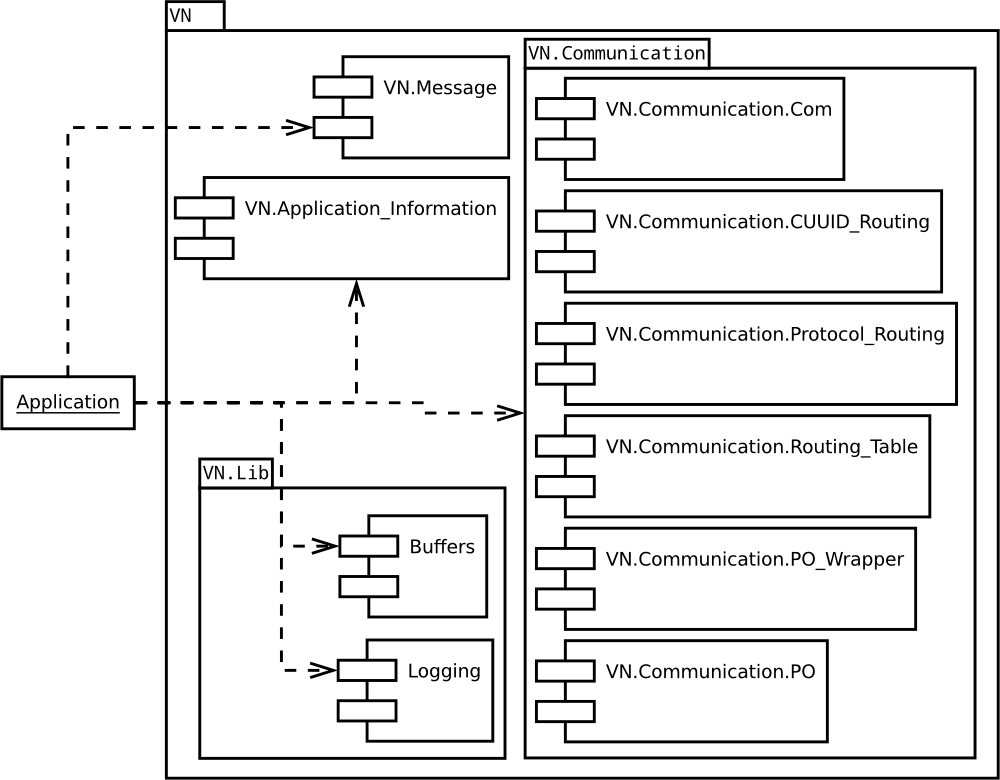
\includegraphics[width=\textwidth]{figures/appendix_component_overview}
    \caption{Component overview of the Virtual Network Library implementation.}
    \label{fig:appendix_component_overview}
\end{figure}

To get one simple application up and running in a "Virtual Network" the
application's settings need to be defined in the \emph{Application\_Information}
component. This ranges from everything from CUUID to other custom settings that
may be needed. The Application\_Information component also keeps track of the
application's logical address during run-time and supplies different helper
functions, one of which is to fill in \emph{VN.Message} header information.

The next step is to add connectivity. If the application only runs on a
processing node or on a single subnet all that is needed is a
\emph{VN.Communication.Com} implementation of that specific subnet type. The
more advanced use case is a subnet manager that manages its own subnet and is
connected to a Local Subnet Manager on the processing node it runs on. As this
requires connectivty on more than one subnet a \emph{Protocol\_Routing} object
will be needed to route traffic between subnets. The Protocol\_Routing object
is a composite type of the VN.Communication.Com interface and can
therefore add multiple subnets during startup procedures.

All communication on a processing node through Ada Protected Objects goes
through the Subnet Manager as a router. This leads to all applications on
a processing node only has to instantiate one connection. This is done by first
instantiating one Protocted Object (PO) through the \emph{VN.Communication.PO}
component. An access to this PO can then be used as input paramter when
creating the two \emph{VN.Communication.PO\_Wrapper's}, one for the application
and one for the local subnet manager.

The application itself is written as an Ada task and due to Ravenscar
limitiation must be built from the ground up for each new task. Best way to
start is to copy an example task from the "examples" directory in the
repository \cite{web:github-vn-lib}.

\section{Component and Service discovery process}\label{sec:discovery_process}
The following sequence diagrams show the basic component and service discovery
process for a local subnet using UDP/IP for inter-process communication
described in SPA Local Subnet Adaptation Draft \cite{spa:local-subnet} (the
sequence of messages sent back and forth is the same for a Local Subnet with
Ada protected objects).

Figure
\ref{fig:appendix_vn_discovery_overview} starts with the high-level view of a
complete SPA network. Figure
\ref{fig:appendix_vn_local_subnet_network_discovery} continues with the
specifics of a SPA Local Subnet. Figure
\ref{fig:appendix_vn_address_block_assignment} shows the specifics on how a SPA
Subnet Manager aquires an address block from the CAS and after that the SPA
Subnet Manager assigns a logical address to each component it is aware of in
figure \ref{fig:appendix_vn_local_subnet_address_assignment}. The last step is the
component capabilities discovery process where the LS collects
information about all known components on the network, this is shown in figure
\ref{fig:appendix_vn_component_capabilities_discovery}.

\begin{figure}[h]
    \centering
    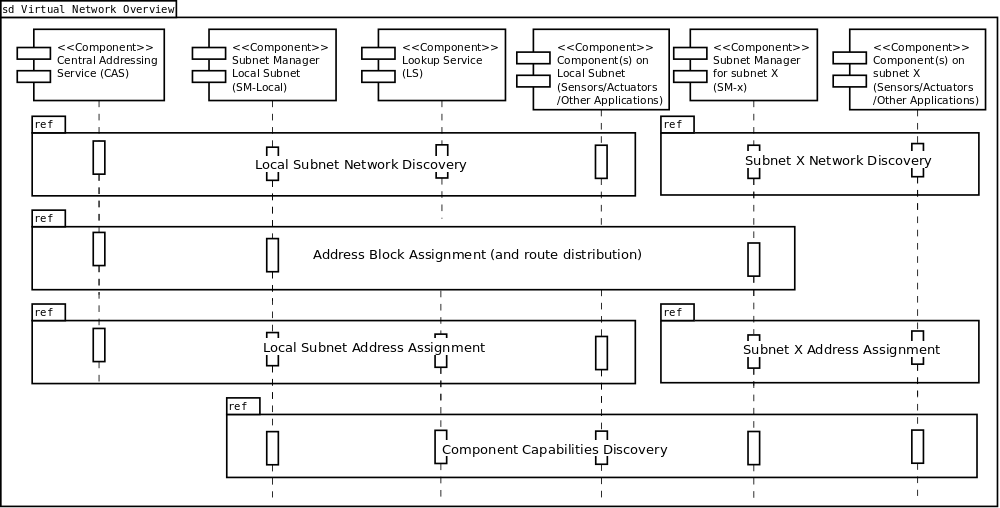
\includegraphics[width=\textwidth]{figures/vn_discovery_overview}
    \caption{Overview of the discovery process for a SPA network.}
    \label{fig:appendix_vn_discovery_overview}
\end{figure}

\begin{figure}[h]
    \centering
    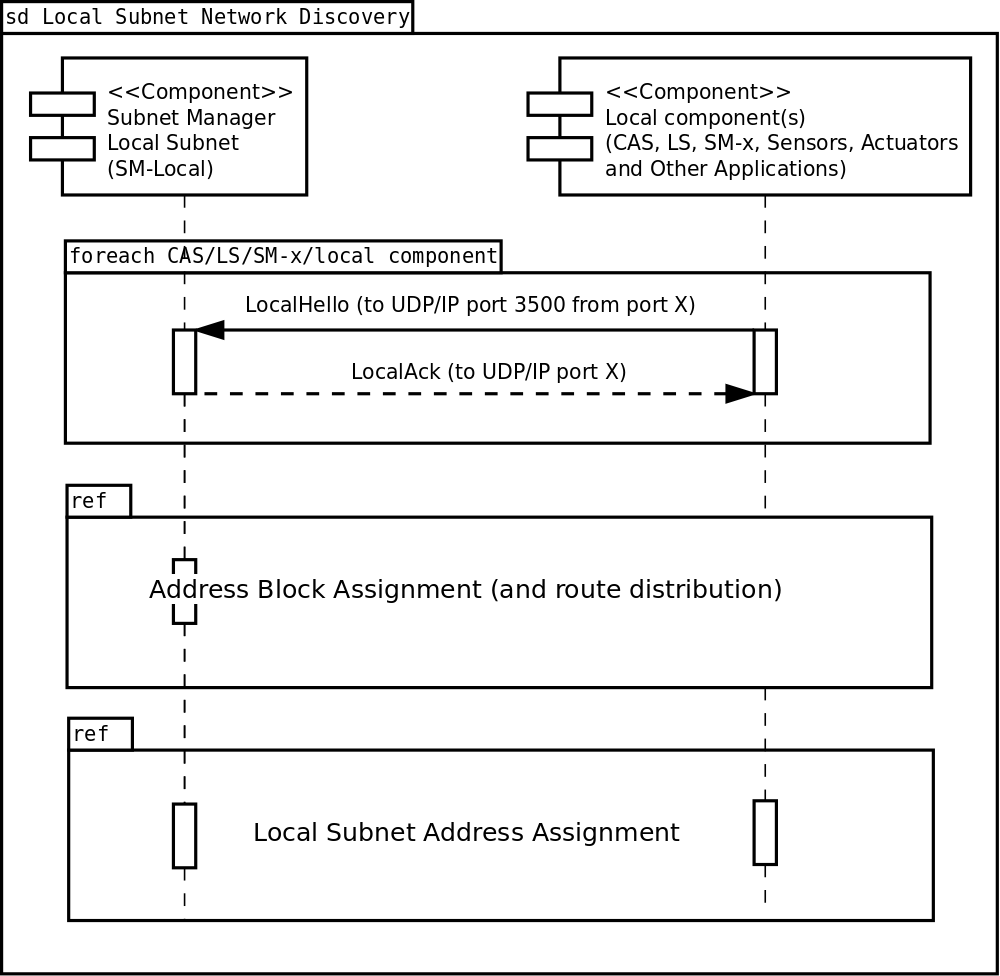
\includegraphics[width=\textwidth]{figures/vn_local_subnet_network_discovery}
    \caption{The basic discovery process for a SPA Local Subnet.}
    \label{fig:appendix_vn_local_subnet_network_discovery}
\end{figure}

\begin{figure}[h]
    \centering
    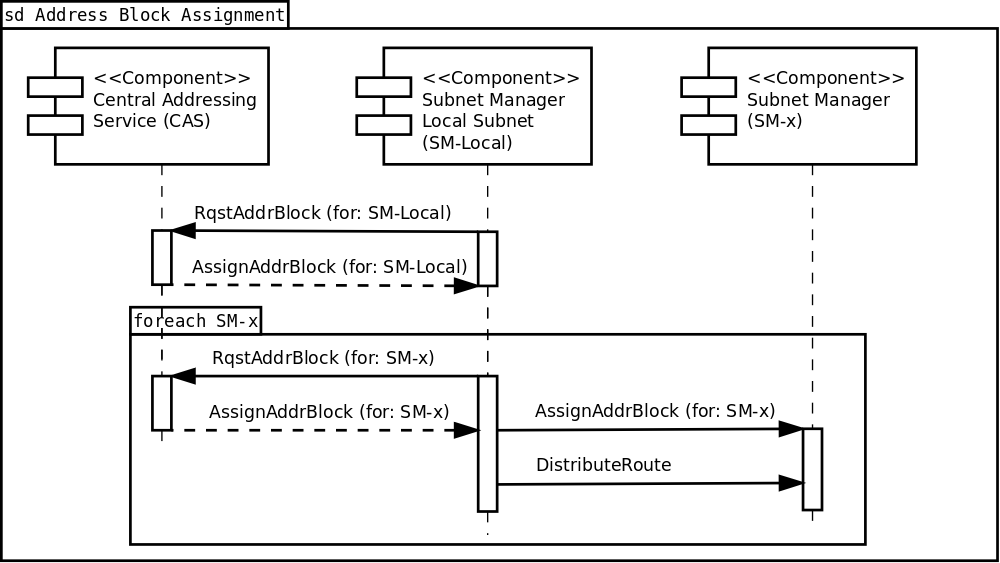
\includegraphics[width=\textwidth]{figures/vn_address_block_assignment}
    \caption{How the local subnet manager aquires address blocks from the CAS
    for its own subnet and for other connected subnet managers.}
    \label{fig:appendix_vn_address_block_assignment}
\end{figure}

\begin{figure}[h]
    \centering
    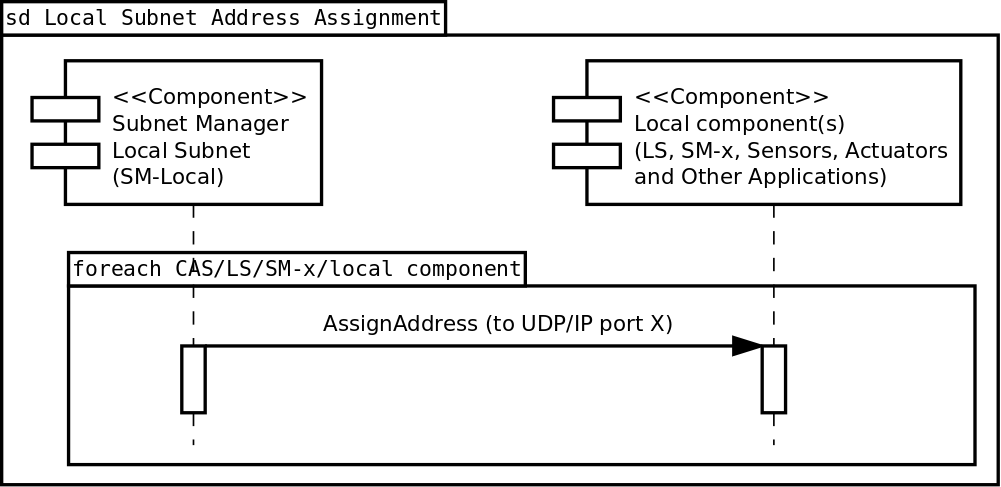
\includegraphics[width=\textwidth]{figures/vn_local_subnet_address_assignment}
    \caption{After the SM-L has received Address Block it starts to assign
    logical addresses to local components it is aware of.}
    \label{fig:appendix_vn_local_subnet_address_assignment}
\end{figure}

\begin{figure}[h]
    \centering
    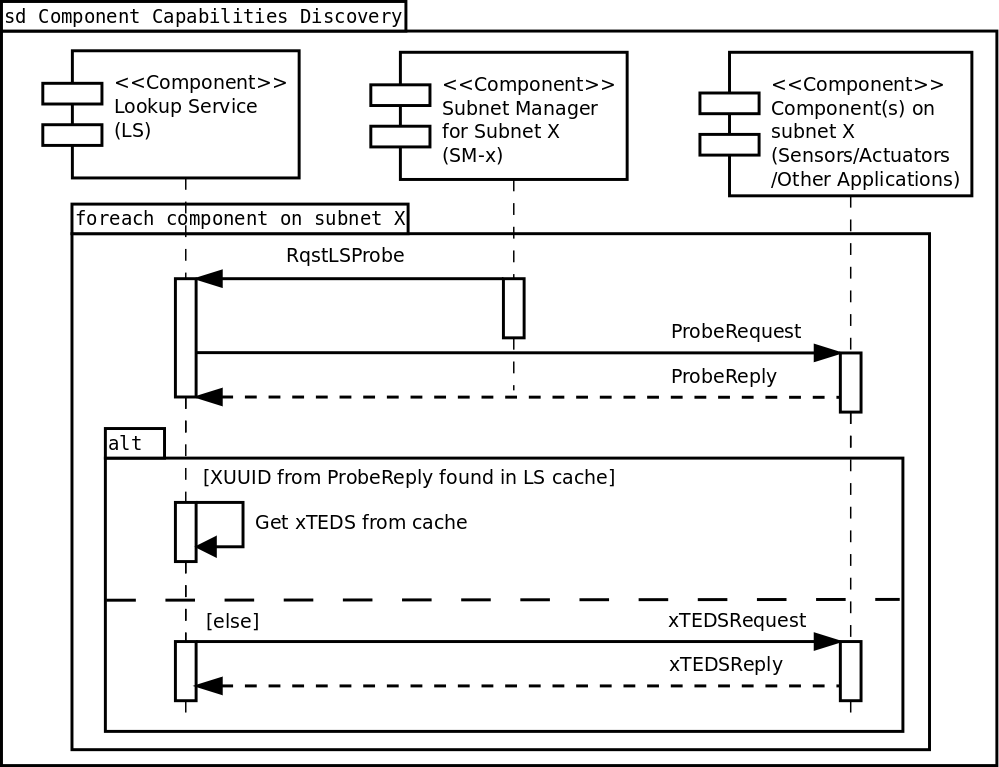
\includegraphics[width=\textwidth]{figures/vn_component_capabilities_discovery}
    \caption{The last step in the discovery process is to discover which
    components have which services.}
    \label{fig:appendix_vn_component_capabilities_discovery}
\end{figure}

% \chapter{UPPAAL Models}

\section{Main UPPAAL model}
TODO: Add the complete set of UPPAAL models used in the end.

TODO: Is this appendix needed or will all UPPAAL models fit in the report?

% \chapter{LaTeX examples}

\section{Example of abbrevations}
This is a short example of abbreviations are added to the list of abbrevations.
The term Fig.\nomenclature{Fig.}{Figure} is now in the List of abbrevations.
The term Img.\nomenclature{Img.}{Image} is now in the List of abbrevations.
The term Tab.\nomenclature{Tab.}{Table} is now in the List of abbrevations.
The term Long Name.\nomenclature{Long Name Long Name}{This is an example of a long
abbrevation that has an even longer description that will hopefully span at
least two rows.} is now in the List of abbrevations.


\section{Figures and images}
Lorem ipsum dolor sit amet, consectetur adipiscing elit. Sed nec ligula vel
ante placerat dapibus. Vestibulum non sollicitudin tellus. Sed varius
vestibulum libero, in euismod purus dapibus sed. Pellentesque malesuada, urna
nec lobortis egestas, felis elit varius ante, in tincidunt nunc metus id diam.
Morbi sagittis velit at ipsum sodales, in tempor nulla volutpat. Integer a
neque eros. In ipsum erat, pellentesque at dapibus eget, pretium sed risus.
Vivamus quis metus vitae felis tempus vulputate eget id lacus. Aenean sit amet
gravida quam, et ornare erat. Praesent ullamcorper mattis dolor, non interdum
orci aliquam a. In tincidunt semper lectus. Duis quis mi ac felis vehicula
mollis. Fusce molestie arcu urna, a tempor turpis mattis nec. Aenean in massa a
risus euismod aliquet vel non libero.

\subsection{One figure}

\begin{figure}[h]
    \centering
    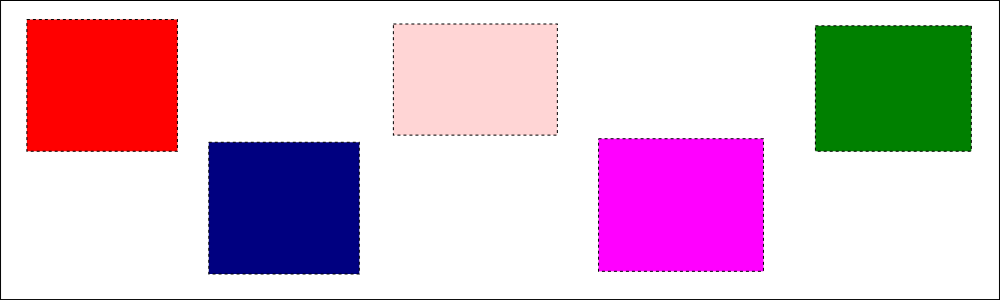
\includegraphics[width=\textwidth]{figures/test_image}
    \caption{Test Image}
    \label{fig:test_image}
\end{figure}

Aenean luctus quam ut neque viverra, quis vulputate mi hendrerit. Nunc id leo
id dui semper blandit. Nulla orci ligula, posuere non lacinia non, aliquet non
massa. Quisque gravida in mi eget volutpat. Fusce convallis felis sed dolor
ornare rhoncus. Nullam sed lacus id lectus venenatis pulvinar eget ac arcu. Sed
id turpis in leo sollicitudin euismod nec ac enim. Nunc vitae lacus lectus.
Class aptent taciti sociosqu ad litora torquent per conubia nostra, per
inceptos himenaeos. Figure \ref{fig:test_image}, Integer gravida, orci vitae
viverra ullamcorper, quam libero tempor est, non gravida magna eros id augue.
In lobortis et est auctor congue. Aliquam sed ante lacus. Vestibulum aliquam
elit eget elementum facilisis. Quisque eget felis eu leo pharetra pharetra.

\subsection{Two sub-figures}
Nulla at purus volutpat, accumsan arcu eget, commodo felis. Cras consequat
risus at rhoncus pellentesque. Aliquam tempor sodales purus in sodales. Sed ut
augue lobortis, mattis felis a, ultricies ante. Pellentesque ac tristique
ipsum, aliquet fermentum ipsum. Sed vel elit sed odio vestibulum semper id eget
enim. Nulla sed hendrerit tortor. Aliquam quam nisl, tempor ut nisl vel,
tristique facilisis libero. Suspendisse id rutrum ante. Duis sed luctus sapien.
Nullam sed quam justo.
\begin{figure}[h]
    \begin{subfigure}[b]{0.5\linewidth}
        \centering
            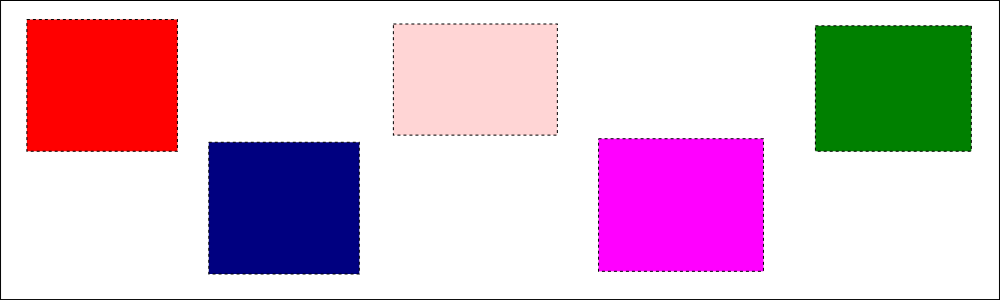
\includegraphics[width=0.9\textwidth]{figures/test_image}
            \caption{This is the caption of Sub-figure 11}
            \label{fig:subfig11}
            \end{subfigure}%
        \begin{subfigure}[b]{.5\linewidth}
            \centering
            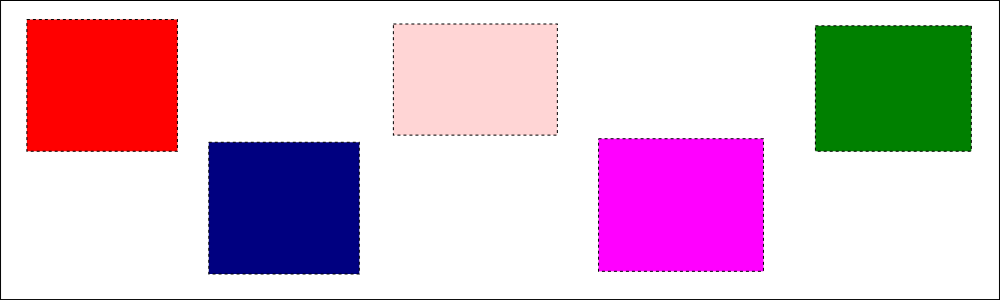
\includegraphics[width=0.9\textwidth]{figures/test_image}
            \caption{This is the caption of Sub-figure 12}
            \label{fig:subfig12}
        \end{subfigure}
    \caption{Two sub-figures}
\label{fig:sub-figures2}
\end{figure}

\subsection{Three figures together on a seperate page for floats}
Nulla at purus volutpat, accumsan arcu eget, commodo felis. Cras consequat
risus at rhoncus pellentesque. Aliquam tempor sodales purus in sodales. Sed ut
augue lobortis, mattis felis a, ultricies ante. Pellentesque ac tristique
ipsum, aliquet fermentum ipsum. Sed vel elit sed odio vestibulum semper id eget
enim. Nulla sed hendrerit tortor. Aliquam quam nisl, tempor ut nisl vel,
tristique facilisis libero. Suspendisse id rutrum ante. Duis sed luctus sapien.
Nullam sed quam justo.

\begin{figure}[p]
    \centering
    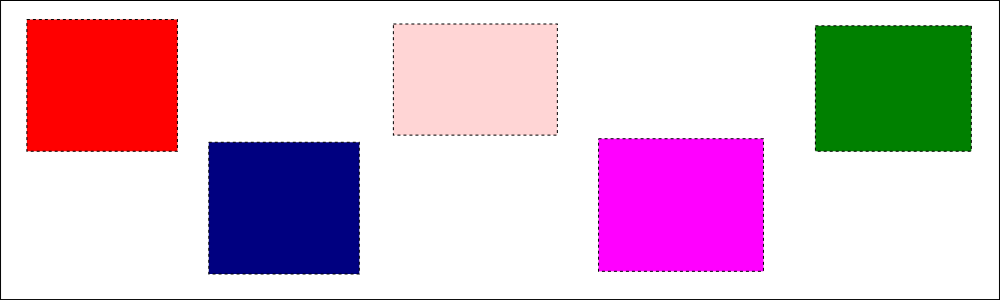
\includegraphics[width=\textwidth]{figures/test_image}
    \caption{Test Image 3}
    \label{fig:test_image3}
\end{figure}

\begin{figure}[p]
    \centering
    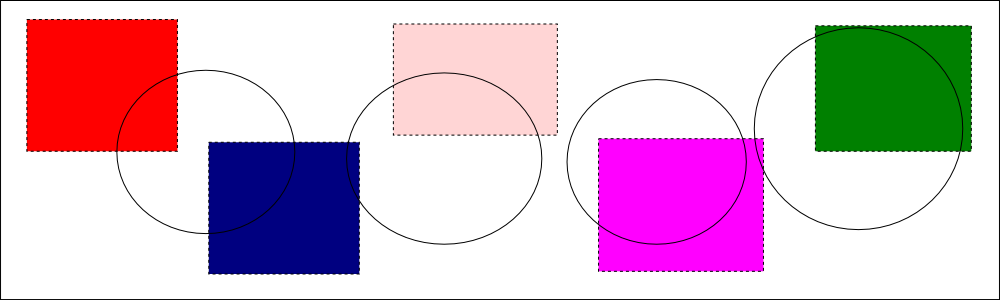
\includegraphics[width=\textwidth]{figures/test_image2}
    \caption{Test Image 4}
    \label{fig:test_image4}
\end{figure}

\begin{figure}[p]
    \centering
    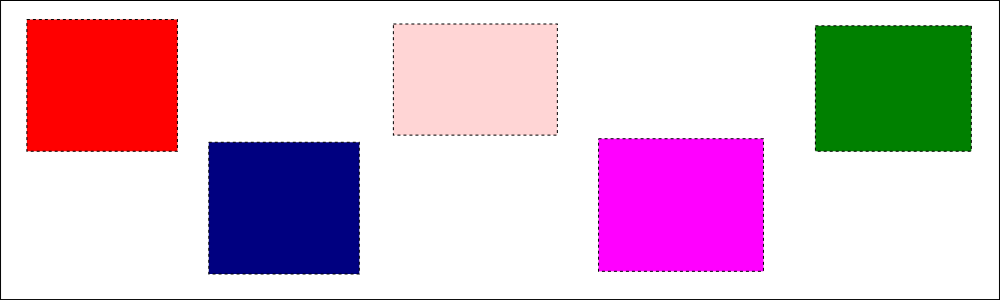
\includegraphics[width=\textwidth]{figures/test_image}
    \caption{Test Image 5}
    \label{fig:test_image5}
\end{figure}

% For more information about tables go to
% https://en.wikibooks.org/wiki/LaTeX/Tables
\section{Tables}
\subsection{One table}
Table \ref{tab:testtab2}, Aenean luctus quam ut neque viverra, quis vulputate
mi hendrerit. Nunc id leo id dui semper blandit. Nulla orci ligula, posuere non
lacinia non, aliquet non massa. Quisque gravida in mi eget volutpat. Fusce
convallis felis sed dolor ornare rhoncus. Nullam sed lacus id lectus venenatis
pulvinar eget ac arcu. Sed id turpis in leo sollicitudin euismod nec ac enim.
Nunc vitae lacus lectus.  Class aptent taciti sociosqu ad litora torquent per
conubia nostra, per inceptos himenaeos. Integer gravida, orci vitae viverra
ullamcorper, quam libero tempor est, non gravida magna eros id augue. In
lobortis et est auctor congue. Aliquam sed ante lacus. Vestibulum aliquam elit
eget elementum facilisis. Quisque eget felis eu leo pharetra pharetra.

\begin{table}[!ht]
  \centering
  \begin{tabular}{l*{6}{c}r}
      Team              & P & W & D & L & F  & A & Pts \\
      \hline
      Manchester United & 6 & 4 & 0 & 2 & 10 & 5 & 12  \\
      Celtic            & 6 & 3 & 0 & 3 &  8 & 9 &  9  \\
      Benfica           & 6 & 2 & 1 & 3 &  7 & 8 &  7  \\
      FC Copenhagen     & 6 & 2 & 1 & 3 &  5 & 8 &  7  \\
  \end{tabular}
  \caption{A floating test table.}
  \label{tab:testtab1}
\end{table}

\subsection{Two tables next to each other}
Some references to the tables on the next page, Table \ref{tab:testtab3} and
Table \ref{tab:testtab4} are sub-tables of Table \ref{tab:testtab2}. Aenean
luctus quam ut neque viverra, quis vulputate mi hendrerit. Nunc id leo id dui
semper blandit. Nulla orci ligula, posuere non lacinia non, aliquet non massa.
Quisque gravida in mi eget volutpat. Fusce convallis felis sed dolor ornare
rhoncus.

\begin{table}[!htb]
    \begin{subtable}{.5\linewidth}
      \centering
        \begin{tabular}{|r|l|}
            \hline
            7C0 & hexadecimal \\
            3700 & octal \\ \cline{2-2}
            11111000000 & binary \\
            \hline \hline
            1984 & decimal \\
            \hline
        \end{tabular}
        \caption{Caption for the first sub-table}
        \label{tab:testtab3}
    \end{subtable}%
    \begin{subtable}{.5\linewidth}
      \centering
        \begin{tabular}{|r|l|}
            \hline
            7C0 & hexadecimal \\
            3700 & octal \\ \cline{2-2}
            11111000000 & binary \\
            \hline \hline
            1984 & decimal \\
            \hline
        \end{tabular}
        \caption{Caption for the second sub-table}
        \label{tab:testtab4}
    \end{subtable}
    \caption{Caption for both tables}
    \label{tab:testtab2}
\end{table}

\subsection{One table with fixed column width}
Aenean luctus quam ut neque viverra, quis vulputate mi hendrerit. Nunc id leo
id dui semper blandit. Nulla orci ligula, posuere non lacinia non, aliquet non
massa. Quisque gravida in mi eget volutpat. Fusce convallis felis sed dolor
ornare rhoncus. Nullam sed lacus id lectus venenatis pulvinar eget ac arcu. Sed
id turpis in leo sollicitudin euismod nec ac enim. Nunc vitae lacus lectus.
Class aptent taciti sociosqu ad litora torquent per conubia nostra, per
inceptos himenaeos. Integer gravida, orci vitae viverra ullamcorper, quam
libero tempor est, non gravida magna eros id augue. In lobortis et est auctor
congue. Aliquam sed ante lacus. Vestibulum aliquam elit eget elementum
facilisis. Quisque eget felis eu leo pharetra pharetra.

\begin{table}[!ht]
  \centering
    \begin{tabular}{ | l | l | l | p{5cm} |}
    \hline
    Day & Min Temp & Max Temp & Summary \\ \hline
    Monday & 11C & 22C & A clear day with lots of sunshine.
    However, the strong breeze will bring down the temperatures. \\ \hline
    Tuesday & 9C & 19C & Cloudy with rain, across many northern regions. Clear spells
    across most of Scotland and Northern Ireland,
    but rain reaching the far northwest. \\ \hline
    Wednesday & 10C & 21C & Rain will still linger for the morning.
    Conditions will improve by early afternoon and continue
    throughout the evening. \\
    \hline
    \end{tabular}
  \caption{A floating test table with fixed column width.}
  \label{tab:testtab6}
\end{table}


\end{document}
